\section{Preliminary on Co-teaching}
Co-teaching~\cite{coteaching} is one of the state-of-the-art approaches for image classification under noisy labels, and can be used to train deep networks robustly even with extremely noisy labels.
It is based on the small-loss concept, i.e. deep models can memorize easy instances first, and gradually adapt to hard instances as training progresses~\cite{memorization}. 
The assumption is that the instances corrupted by label noise are hard for the network to learn, while the clean ones are comparatively easy. 

Specifically, two networks $P$ (with parameter $w^1$) and $Q$ (with parameters $w^2$) are maintained. 
For a mini-batch $\mathcal{D}$ (step 5), the networks $P$ (resp. $Q$) selects a small proportion of instances from this mini-batch $\mathcal{D}^1$ (resp. $\mathcal{D}^2$) that have small training loss (steps 6 and 7). 
The number of instances is controlled by $R(T)$, and $P$ (resp. $Q$) only selects $R(T)$ percentage of small loss instances out of the mini-batch. Then, the selected instances are fed into its peer network as the useful knowledge for parameter updates (steps 8 and 9).
In the training procedure, $R(T)$ is used (at epoch $T$) to quantify the amount of small loss
samples per mini-batch to be used to update the network weights. $R(T)$ is directly related
to the amount of label corruption $\epsilon$ ($\epsilon$ is assumed to be known), and is defined as $R(T)= 1- \min\bigg\{\dfrac{T}{T_k}\epsilon, \epsilon\bigg\}$, where $T_k$ is the epoch after which $R(T)$ becomes constant. Typical profiles of $R(T)$ for different $\epsilon$ is shown in Figure \ref{fig:R(T)}. In algorithm 1, we observe that the model initially considers all the input data and slowly zones into the cleanly labeled data (guided by the concept of small loss instances) to train the model. After completion of $T_k$ epochs ($T_k$: hyperparameter), the network weights are updated using $(1 - \epsilon)$ portion of the training data (marked as small loss instances) and ignores the large loss samples under the assumption that they are wrongly labeled.
\begin{figure}[ht]
            \centering
            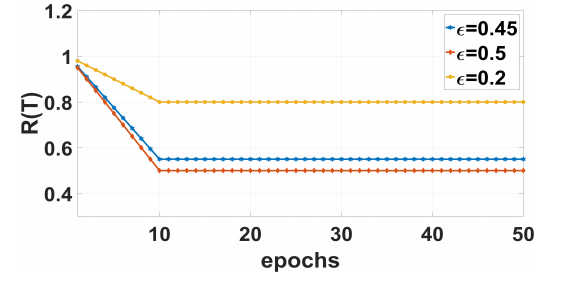
\includegraphics[scale = 0.5]{plot_R(T).png}
            \caption{Plot of $R(T)$ for different values of label corruption $\epsilon =\{0.45,0.5,0.2\}$ and $T_k = 10$. $R(T)$ is used \cite{coteaching} to control how many samples are used to update the network weights per epoch.}
\label{fig:R(T)}
\end{figure}
\begin{algorithm}[H]
	\caption{Co-teaching Algorithm.} 
	\begin{algorithmic}[1]
	    \State \textbf{Input:} $w^1$ and $w^2$, learning rate $\eta$, fixed $\epsilon$, epoch $T_k$ and $T_{max}$, iteration $N_{max}$;
		\For {$T=1,2,\ldots, T_{max}$}
		    \State Training set ${D}$;
			    \For {$N=1,2,\ldots, N_{max}$}
				    \State \textbf{Fetch} mini batch $\mathcal{D}$ from ${D}$
				    \State \textbf{Obtain} $\mathcal{D}^1 = \argmin_{\mathcal{D}':|\mathcal{D}'|\geq R(T)|\mathcal{D}|} \mathcal{L}(P, \mathcal{D}')$   \Comment{$\mathcal{L}$: cross entropy loss}
				    \State \textbf{Obtain} $\mathcal{D}^2 = \argmin_{\mathcal{D}':|\mathcal{D}'|\geq R(T)|\mathcal{D}|} \mathcal{L}(Q, \mathcal{D}')$
				    \State \textbf{Obtain} $L^1(w^1) = \mathcal{L}(P,\mathcal{D}^2)$ \Comment{Loss for network 1: $P$}
				    \State \textbf{Obtain} $L^2(w^2) = \mathcal{L}(Q,\mathcal{D}^1)$ \Comment{Loss for network 2: $Q$}
				    \State \textbf{Update} $w^1 = w^1 - \eta \nabla L^1(w^1)$
				    \State \textbf{Update} $w^2 = w^2 - \eta \nabla L^2(w^2)$
			    \EndFor
			 \State \textbf{Update} $R(T)= 1- \min\bigg\{\dfrac{T}{T_k}\epsilon, \epsilon\bigg\}$
		\EndFor
	\end{algorithmic} 
\end{algorithm}


When the test data follows similar distribution as the training data, Co-teaching will steadily improve learning. 
%However, when the test data has a distribution shift from the training data, the existing curriculum will be less specified. 
But in the problem addressed, due to the distribution shift, the test data will be substantially dissimilar to the training data. 
Thus, even if the training samples with smaller loss are noise-free, they are not necessarily relevant to the learning task of the test data.